\documentclass{standalone}
\usepackage[utf8]{inputenc}
\usepackage{tikz}
\usetikzlibrary{calc,patterns,angles,quotes}
\begin{document}

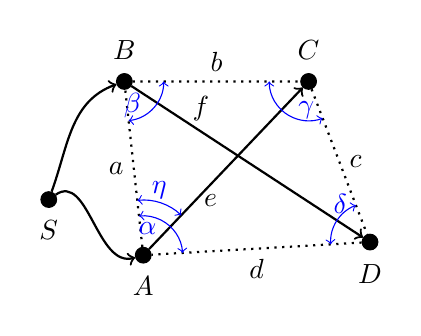
\begin{tikzpicture}[scale=.6]
% \draw[rounded corners=5mm, fill=gray!20, draw=white] (-.7,-.2) -- (3.5,0.7) -- (0.2,4.5) -- cycle;
%  \node[label={[gray]$T_{i_1/i}$}] (Ti1i) at (2,2) {}; 
  \begin{scope}[every node/.style={circle,draw=black,fill= black,minimum size=3.5pt, inner sep=2}];
  \node[label=below:$S$] (S) at (0,0) {};
  \node[label=below:$A$,below] (A) at (2,-1) {};
  \node[label=$B$] (B) at (1.6,2.5) {};
  \node[label=$C$] (C) at (5.5,2.5) {};
  \node[label=below:$D$ ] (D) at (6.8,-0.9) {};
  \end{scope}
	\draw[thick,->] (S) to[out=35, in=196]  (A);
	\draw[thick,->] (A) -- (C) node[pos=0.4,below] {$e$}; 
	\draw[thick,->] (S) to[out=70, in=200] (B);
	\draw[thick,->] (B) -- (D) node[pos=0.3,above] {$f$}; 
	\draw[thick,dotted] (A) -- (B) node[pos=0.5,left] {$a$};
	\draw[thick,dotted] (B) -- (C) node[pos=0.5,above] {$b$};
	\draw[thick,dotted] (C) -- (D) node[pos=0.5,right] {$c$};
	\draw[thick,dotted] (D) -- (A) node[pos=0.5,below] {$d$};
	\pic [draw=blue, <->, text=blue,"$\alpha$",angle eccentricity=0.9,left] {angle = D--A--B};
	\pic [draw=blue, <->, text=blue,"$\beta$",angle eccentricity=0.9,above,left] {angle = A--B--C};
	\pic [draw=blue, <->, text=blue,"$\gamma$",angle eccentricity=0.9, right] {angle = B--C--D};
	\pic [draw=blue, <->, text=blue,"$\delta$",angle eccentricity=0.9,right, above] {angle = C--D--A};
	\pic [draw=blue, <->, text=blue,"$\eta$",angle eccentricity=0.9,right, above, scale=1.4] {angle = C--A--B};
  \end{tikzpicture}
  \end{document}
